\documentclass[conference,compsoc]{IEEEtran}

\ifCLASSOPTIONcompsoc
  \usepackage[nocompress]{cite}
\else
  % normal IEEE
  \usepackage{cite}
  \usepackage{graphicx}
  \usepackage{graphicx}
  \usepackage{url}
  \usepackage[english]{babel}
  \usepackage{times}
  \usepackage{amssymb}
  \usepackage{color}
  \usepackage{xspace}
  \usepackage{listings}
  \usepackage{upquote}
  \usepackage[hidelinks]{hyperref}
  \usepackage{wrapfig}
  \graphicspath{ {/Users/tejasK/Documents/ASU Coursework/FSL/Project/IEEEtran/} }
\fi

\ifCLASSINFOpdf
  \usepackage[pdftex]{graphicx}
   \usepackage{url}
  \usepackage[english]{babel}
  \usepackage{times}
  \usepackage{amssymb}
  \usepackage{color}
  \usepackage{xspace}
  \usepackage{listings}
  \usepackage{upquote}
  \usepackage[hidelinks]{hyperref}
  \usepackage{wrapfig}
  \graphicspath{ {/Users/tejasK/Documents/ASU Coursework/FSL/Project/IEEEtran/} }

\else

  \usepackage[dvips]{graphicx}
   \usepackage{url}
  \usepackage[english]{babel}
  \usepackage{times}
  \usepackage{amssymb}
  \usepackage{color}
  \usepackage{xspace}
  \usepackage{listings}
  \usepackage{upquote}
  \usepackage[hidelinks]{hyperref}
  \usepackage{wrapfig}
  \graphicspath{ {/Users/tejasK/Documents/ASU Coursework/FSL/Project/IEEEtran/} }
\fi

\hyphenation{op-tical net-works semi-conduc-tor}


\begin{document}

\title{Multiple Instances Learning - EMDD}

\author{\IEEEauthorblockN{Tejas Khairnar}
\IEEEauthorblockA{Arizona State University\\
Email: tkhairna@asu.edu}
\and
\IEEEauthorblockN{Vivin Paliath}
\IEEEauthorblockA{Arizona State University\\
Email: tkhairna@asu.edu}}

\maketitle

\begin{abstract}
In this midterm report for CSE 569 Fundamentals of Statistical Learning we are trying to perform Image categorization using Estimation Maximization Diverse Density Algorithm(EMDD). Multiple-Instances Learning (MIL) is a generalization of the supervised learning classification problem. Using EMDD algorithm we classify the instances in the given data set as positive instances or a negative instance. [Our algorithm calculates the probability of the instance to be a positive or negative instance].
\end{abstract}


\IEEEpeerreviewmaketitle



\section{Introduction}
% no \IEEEPARstart
Multiple Instances Learning (MIL) is proposed as a variation of supervised learning for problems with incomplete knowledge about labels of training examples. In supervised learning, every training instance is assigned with a discrete or real-valued label. In MIL the labels are only assigned to bags of instances. In the binary case, a bag is labeled positive if at least one instance in that bag is positive, and the bag is labeled negative if all the instance in it are negative There are no labels on the individual instances. The goal of MIL is to classify unseen bags or instances based on the labeled bags as the training data. For this specific project we focus on EMDD algorithm to perform the traning and categorization~\cite{chen2004image}. However, we also compare this implementation of ours with various other implementations of MIL algorithms.

\section{Understanding}
\subsection{Diverse Density Algorithm}
The main idea of DD approach is to find a concept point in the feature space that are close to at-least one instance from every positive bag and meanwhile far away from instances in negative bags~\cite{MILlink}. The optimal concept point is defined as the one with maximum density, which is a measure of how many different positive bags have instances near the point, and how far the negative instances are from that point.
\subsection{Estimation Maximization}
The Estimation Maximization algorithm is an effective iterative procedure to compute the Maximum Likelihood (ML) estimate in the presence of missing or hidden data~\cite{EMlink}. In ML estimation, we wish to estimate the model parameter(s) for which the observed data are the most likely.
Each iteration of the EM algorithm consists of two processes: The E-step, and the M-step. In the expectation, or E-step, the missing data are estimated given the observed data and current estimate of the model parameters. This is achieved using the conditional expectation, explaining the choice of terminology. In the M-step, the likelihood function is maximized under the assumption that the missing data are known. The estimate of missing data from the E-step are used in lieu of the actual missing data.
Convergence is assured since the algorithm is guaranteed to increase the likelihood at each iteration.
\subsection{EMDD}
EM-DD~\cite{MILlink} starts with an initial guess of the concept point t (which can be obtained using original DD algorithm), and then repeatedly performs the following two steps: E-step, the current hypothesis of concept t I used to pick the most likely instances from each bag given a generative model; in M-step, a new concept t’ is estimated by maximizing a transformed DD defined on the instances selected in the E-step using the gradient search. Then, the old concept t is replaced by the new concept t’ and the two steps are repeated until the algorithm converges. This EM-DD algorithm which we have implemented, implementes a “hard” version of EM, since only one instance per bag is used for estimating the hypothsis. It can be also regarded as a special case of the K-means clustering algorithm~\cite{Harti} , where only on cluster is considered.

\section{Progress}
Until midterm, we have successfully implemented the EMDD algorithm in python programming language. In order to perform the Math behind the algorithm we are using the SciPy library~\cite{Scipy}. According to the goals allocated for this project, we have tested our implementation against the Synthetic data set~\cite{SynthDataset}. In order to perform the comparison of results obtained by our implementation and the Matlab implementation of MIL algorithms ~\cite{MILlink}, we performed the Matlab setup and ran the Matalb setup for algorithms like 
\begin{itemize}
	\item Iterated-discrim APR
	\item Diverse Density
	\item Two SVM variants for MIL
	\item Citation-kNN for MIL
\end{itemize}
Currently we have the results for these algorithms against the Synthetic dataset. We are now in progress of moving toward the public dataset list ~\cite{MILlink,andrews2002support,Lichman:2013}.

\section{Timeline}
Below is the timeline for this project which we chalked out:
\begin{figure}[t]
	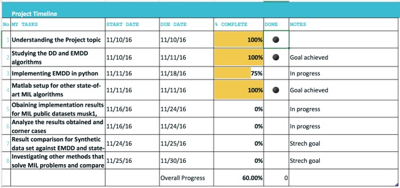
\includegraphics{timeline}
\end{figure}


\section{Results}
We don not need to put in results for our midterm report.

\section{Workload Shared}
The workload amongst us was shared equally. We worked together on the implementation. The major part of coding was done by Vivin and I took care of the Matlab setup and result comparison part. 


\section{Conclusion}
Till midterm we have successfully completed the task mentioned. We are focusing on achieving all the goals mentioned in the timeline.



% conference papers do not normally have an appendix



% use section* for acknowledgment
\ifCLASSOPTIONcompsoc
  % The Computer Society usually uses the plural form
  \section*{Acknowledgments}
\else
  % regular IEEE prefers the singular form
  \section*{Acknowledgment}
\fi


The authors would like to thank...

\bibliographystyle{abbrvnat}
\bibliography{main}{}

\end{document}


